%% LyX 2.2.3 created this file.  For more info, see http://www.lyx.org/.
%% Do not edit unless you really know what you are doing.
\documentclass[11pt]{article}
\usepackage[utf8]{inputenc}
\setcounter{secnumdepth}{2}
\usepackage{amsmath}
\usepackage{amssymb}
\usepackage{graphicx}
\usepackage{hyperref}

\makeatletter
%%%%%%%%%%%%%%%%%%%%%%%%%%%%%% User specified LaTeX commands.
%%AGT class -- Feldman -- TAU -- Spring 2018 %%


    \textwidth=6in
    \oddsidemargin=0.25in
    \evensidemargin=0.25in
    \topmargin=-0.1in
    \footskip=0.8in
    \parindent=0.0cm
    \parskip=0.3cm
    \textheight=8.00in


    \sloppy

    \DeclareMathOperator*{\argmax}{argmax}
    \DeclareMathOperator*{\argmin}{argmin}

\makeatother

\begin{document}
\setlength{\oddsidemargin}{.25in} \setlength{\evensidemargin}{.25in}
\setlength{\textwidth}{6in} \setlength{\topmargin}{-0.4in} \setlength{\textheight}{8.5in}

\global\long\def\handout#1#2#3#4{ \global\long\global\long\global\long\def\thepage{#1-\arabic{page}}
\noindent\begin{center} \framebox{ \vbox{ \hbox to 6.35in { {\bf Advanced Topics in Multi-Core Architecture and Software Systems} \hfill#1 } \vspace{4mm} \hbox to 5.78in { {\Large\hfill#4 \hfill} } \vspace{2mm} \hbox to 6.35in { {\it #2 \hfill#3} } } } \end{center} \vspace*{4mm} }

\global\long\def\finalProjTitle#1#2#3#4{\handout{#1}{Lecturer: #2}{Names: #3}{#4}}

\newtheorem{theorem}{Theorem} \newtheorem{corollary}[theorem]{Corollary}
\newtheorem{lemma}[theorem]{Lemma} \newtheorem{observation}[theorem]{Observation}
\newtheorem{proposition}[theorem]{Proposition} \newtheorem{definition}[theorem]{Definition}
\newtheorem{claim}[theorem]{Claim} \newtheorem{fact}[theorem]{Fact}
\newtheorem{assumption}[theorem]{Assumption} \newtheorem{example}{Example}

\global\long\def\qed{\rule{7pt}{7pt}}

\newenvironment{proof}{\noindent{\bf Proof:}\hspace*{1em}}{\qed\bigskip}
\newenvironment{proof-sketch}{\noindent{\bf Sketch of Proof:}\hspace*{1em}}{\qed\bigskip}
\newenvironment{proof-idea}{\noindent{\bf Proof Idea:}\hspace*{1em}}{\qed\bigskip}
\newenvironment{proof-of-lemma}[1]{\noindent{\bf Proof of Lemma #1:}\hspace*{1em}}{\qed\bigskip}
\newenvironment{proof-attempt}{\noindent{\bf Proof Attempt:}\hspace*{1em}}{\qed\bigskip}
\newenvironment{proofof}[1]{\noindent{\bf Proof}
    of #1:\hspace*{1em}}{\qed\bigskip} \newenvironment{remark}{\noindent{\bf Remark}\hspace*{1em}}{\bigskip}

%%%%%%%%%% My additions
\global\long\def\fakebold#1{\ThisStyle{\ooalign{$\SavedStyle#1$\cr%
\kern -\bshft$\SavedStyle#1$\cr%
\kern \bshft$\SavedStyle#1$}}}

%%%%%%%%%%%%%%%%%%%%%%%%%%%%%%%%%%%%%%%%%%%%%%%%%%%%%%%%%%%%%%%%%%%%%%%%%%%%%%%%%%%%%
%%Michal%% ==> Change the lecture number, lecture date, and Scribe name
\finalProjTitle{March 17, 2019}{Dr. Adam Morrison}{Liad Aben
Tzur, Sapir Freizeit and Almog Freizeit}{Transactional Data Structures}

%%Michal%%  Name the first section.  You can then use more sections (and, if needed, subsections)
\begin{abstract}
The idea of transactional data structures is to enable performing
complex atomic transactions. It is widely used in many software and
algorithms which use parallelism. Usually these kind of data structures
are performance oriented and therefore a high-performance implementation
for it is a novel cause. There exists a paper trying to address this
point \cite{TDSL}, yet for now only a
java implementation exists for it (\url{https://github.com/HagarMeir/transactionLib}), which is buggy
and use GC which affects performance. Therefore, our main goal in
this project was to implement a C++ version of it, using memory reclamation.
By doing so we hoped to achieve better results.
\end{abstract}

\section{Transactional Data Structures - TDS}

A transactional data structure is a data structure with its native
operations (such as add or remove in a list and enqueue in a queue),
plus two special operations: \textit{TXBegin} and \textit{TXCommit}.
The library guarantees atomicity for each group of operations executed
in between a TXBegin and a TXCommit (a \textbf{transaction}) – meaning
that either they succeed together, or they will all fail (no partial
results are visible for any other thread). \\
 Our implementation for the library is highly based on the paper \cite{TDSL}. In this paper, the method offered for implementation
is to make each thread have its own read-set and write-set which it
updates inside a transaction. At the end of the transaction, the thread
acquires locks of all the elements in its read/write sets and make
sure it is safe to update all of them. “Safe” is defined via a \textit{global
version clock (GVC)}, where node is safe to be changed if the GVC
observed at the insertion of this node to the write/read sets is equal
to the GVC observed after acquiring its lock. Only if all the nodes
in the set are safe to be changed, the transaction succeeded. Otherwise,
the transaction fails.\\
 In order to minimize the contention between different threads, the
library maintains an Index. The index is basically a concurrent skip-list,
which is always updated only by a successful transaction. When finding
a node in the list, one should go and search for it in the index.
The index guarantee is to return a node which key is less than yours,
and all the requested thread remains to do is to walk from this node
forward, which spreads the threads along the list and minimizes collisions.

\section{Our Implementation}

A Github repository is available here: \\ \url{https://github.com/liadab/TransactionalDataStructures}

\subsection{Changes We Have Made}

While implementing the library in C++ we have made some changes to the original Java implementation we based on. In this section we will describe each of them and the reasons which led to the change.

\subsubsection{Templates}

Each of our node is a template class, which is templated upon both
its key and its value. This method enables flexibility when using
our library yet remains the implementation neat and elegant. \\
 The only demand from the keys is to act like numbers, in the manner
that they have to support the “+”, “-“ operations and the std::numericlimit
function.

\subsubsection{LNodeWrapper}

One of our main goals at the project was to implement the library
in C++ without neglecting memory reclamation in order to support large
data sets. We wanted to compare different methods of memory reclamation,
as well as a leaking algorithm. Therefore, we came up with the \textit{LNodeWrapper}
design. The wrapper enables memory management to be hidden from the
user and to be managed fully by the wrapper. \\
 In that way we could easily test and compare different memory reclamation
models, with as minimum changes as possible, and in a short amount
of time.

\subsubsection{Index}

The index is highly lean on the Java implementation yet have some
changes. In order to fully understand the changes, lets discuss shortly
about the index’s design. \\
 As mentioned before, the index is basically a skip list. Therefore,
it has several different levels, each level starts with a special
node which is the head of the that level’s list. Each index node has
a pointer to the next node in its layer, and a pointer downwards to
the appropriate node on level lower (at the bottom layer this pointer
is NULL). Each index node points also to the real Linked List Node,
where nodes in different levels corresponding to the same LL-node.
\\
 When a new node is added to the index, after its level is chosen
randomly, all of its index nodes at different levels of the skip list
is created, pointed to each other in the “down” pointer. Therefore,
for correctness, one should always insert the new nodes from bottom
level upwards, so that nodes in the index will always point to another
node which is in the index as well. Yet for some reason the Java implementation
made all the nodes in the index, including the head nodes, point only
downwards, so the insertion is performed from top level downwards
as well. This is our first change: we made only the heads a double-linked-list,
meaning that each head has both a pointer downwards and upwards to
the lower and higher levels respectively. Doing so made insertion
from bottom up more elegant yet added some subtle pointes we had to
treat carefully. \\
 Another addition to our index is a function called \textit{“findInsertionPoints”},
which given a node returns all the insertion points for it in all
the different levels (aka two vectors corresponding to the previous
and next node in each level). In that way the contention between different
threads is minimized at insertion as well, other than only at searching.
\\


\subsubsection{Local Storage}
In the java implementation there were a global singleton of local storage, since the java implementation didn’t have multitype support it was o, but in our c++ implementation we needed to be template, so we used the thread local syntax in c++. \\
Thread local in a member function create a copy of the local object for each thread that calls it and that’s exactly what we want. \\
Since the method that contains the local storage is template, we get a local storage for each different key and value we use. \\
The only downside is that because we can't know on which types, we used the local storage we need to call txend on the types we used, so the code would commit the right types.

\subsubsection{Multiple Executables}

In order to compare the different memory reclamation approaches, we
created many different executables, one for each method. The comparison
was made by a different python script which only had to run the different
executables and measure the results. \\
 Therefore it is easy for a user to choose which model he prefer to
use when using our library, depends if he cares more about efficiency
or perhaps he prefer to not approve any memory leak, as small as it
may be.

\subsubsection{Linked List}
Our linked list implementation is quite similar to the java's, algorithm wise. \\
As mentioned above we used the \textit{LNodeWrapper} for node pointers. \\
We also cleaned the code, for example in each method on the Linked List beginning there was some identical operations with key (for example: search for the node with a specific key or the node closest to it).
The java library always copied the same code to find the node and merged the method-specific handling code inside it. We exported out the find logic and that way our Linked List code was much shorter, end easier to understand and debug. \\
Another change we have made regarded unnecessary allocations. The java code allocated nodes sometimes even in cases it shouldn’t have, which was inefficient, so we deleted those unneeded allocations.
Also, there were some bugs that we fixed:
\begin{itemize}
    \item In remove if the node was at the end of the list, the removing logic was incorrect.
    \item There was a bug in the find next logic that there was an abort that should have occurred in case of a singleton intervention that wasn’t handled.
\end{itemize}

Another change we've made is that we add the logic of when we can retire a node in case it was deleted for integrate the Debra implementation in our library.

\subsection{Non-Leaking Algorithm}

One of our main goals at the project was to create a non-leaking implementation in C++, without relying on any garbage collector, yet keeping it efficient and usable in large scales.\\
In order to achieve our goal we tested and compared two main approaches for doing so, the first is based on the standard C++ solution, and the second uses a more specific yet more complex solution. \\
A detailed explanation of the both solutions follows:

\subsubsection{Using Shared Pointers}
We found that using refcount was the easiest way for implementing a working solution to the memory reclamation problem. \\
The idea of shared ptr is that each pointer also has a refcount allocated on the heap, and that way the pointer can know if there are other pointers, which can access it, or if there are no other pointer which can access this pointer and we don’t need it. Therefore it can safetly determine when to delete this memory. \\
That way, using RAII, we could know that there indeed was no memory leakage.\\
While validating it we noticed one unexpected leakage: in the index, due to the fact that we have nade the heades of all the different levels be a doubly-linked-list, there became a situation when two nodes had shared ptrs to each other, remained each other alive. We solved that by breaking these chains manually on the index destractor. \\
The only downsize to this memory reclamation method is that each time we copy a pointer, we need to do fetch and add, and each time we stop we need to do fetch and dec, which can become a bottleneck in large scales.

\subsubsection{Using DEBRA}
DEBRA (\url{https://www.cs.toronto.edu/~tabrown/debra/impl.htm}) is a library which uses the concept that each time we want to access the memory, we declare, using the guard a filter of which memory we can access, Debra does this in O(1), then when we want to delete a node, we retire it, making it in a state of want to be deleted. \\
When the application decides to retire a node, we must make sure manually that each new thread which started after the retire occurred (actually after the guard is out of scope) cant access the node that was retired.\\
Using this assumption when a guard is getting out of context, if it was the last guard that started after that node retired occurred it can safely delete this node.\\
Both guard ctr, dctr and node retire are in o(1) which is very efficient.
Using Debra is the most efficient way we found to do memory reclamation.
Debra downside is in order to use Debra properly the application must be aware to Debra and we must manually retire the nodes and make sure we do the assumptions:
\begin{itemize}
\item Correctly using guards.
\item Make sure that a thread that started a guard after retiring can't access the node.
\end{itemize}
Unlike shared ptr which is plug and play.


\subsection{Concurrent Testing System}

We tested our code using the GTEST unit testing library which enabled us an easy way to run complicated and diverse tests. Mainly, as for every concurrent library, we tried to detect the interesting races that could occur, and clarify our implementation correctness during those ones. \\
A very helpful tool we developed was the \textit{Thread Runner} testing tool. This tool enables control a two threads flow, which enables us create the "race" on our own in order to test it. The idea is to makes a thread run a partial logic, then logically freeze it and enable another thread make another logic, and then end the rest of the original logic. \\
An example for a test we created is making one thread do a transactional put, then freeze it, and another start another thread which do a singleton get for the same key (should not find the node). Then the first thread unfreeze and try to commit, after the commit the other thread is doing singleton get which this time succeed. \\
Using this tool we tested interesting cases and found some bugs in the java implementation we were based on.

\section{Tests and Measurements Environment}

\subsection{Our Running Scenario}

We wrote a similar running scenario for both the Java implementation
mentioned in {[}1{]}, and our C++ implementations:
\begin{enumerate}
\item First, we receive the parameters: amount of threads, amount of total
tasks, amount of tasks per transaction, total percent of insert operations,
and total percent of remove operations (the rest will be search opeartions).
\item We create a pool of random tasks, so the randomization process is
not included in our time measurement.
\item We create a linked list (we use the linked list as our study case)
and initialize it with nodes. By doing that, we start the actual measurement
from a 'clean' environment.
\item We create a bunch of workers in separate threads as the amount of
threads we got. Each worker receives a different section of the tasks
pool from step (2), and a pointer to the linked list we created in
(3), and we let the workers run parallel and perform the tasks from
the pool.
\item In the last stage we print our results.
\end{enumerate}

\subsubsection{notes}
\begin{enumerate}
\item We measure the running time only of step 4 - where the parallel work
is done on the data structure.
\item We use the JAVA implementation from the article as-is, the only thing
we added is the Main file, that executes the scenario described above.
\end{enumerate}

\subsection{Running and Output Examples}

\subsubsection{Running Examples}

We checked 4 implementations:
\begin{align*}
our\ non-leaking\ CPP & ./tds\ 2\ 1000\ 10\ 40\ 50\\
our\ leaking\ CPP & ./tds\_unsafe\ 2\ 1000\ 10\ 40\ 50\\
our\ using-debra\ CPP & ./tds\_debra\ 2\ 1000\ 10\ 40\ 50\\
JAVA\ implementation\ from\ the\ paper & ./run\ 2\ 1000\ 10\ 40\ 50
\end{align*}
Here 2 is the number of threads that will run in parallel, 1000 is
the total number of tasks (each thread will execute 500 tasks), 10
is the amount of tasks per transaction, 40 is the percent of inserts
tasks, and 50 is the percent of remove tasks.\\
Overall we programmed 3 executables: tds, tds\_debra and tds\_unsafe.

\subsubsection{Output Example:}

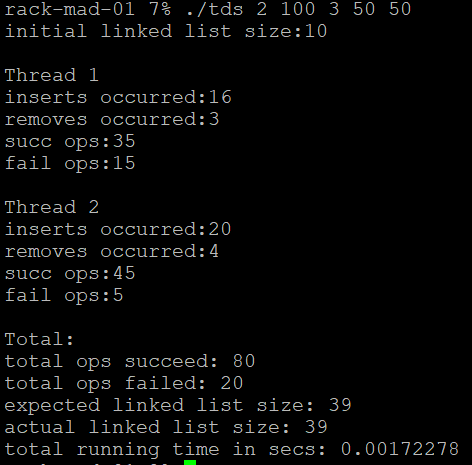
\includegraphics{pasted1}

\subsubsection{Output explanation:}

At the beginning we print the initial size of the linked list. After
the workers are done, for each thread we count the amount of inserts
and removes occurred, meaning inserts and removes that changed the
data structure state. Also, we count the number of successful operations
and the number of failure operations, where here a 'failure' means
that the transaction aborted due to a change in the data structure.
At the end, we print a summary of the details. The output is equal
for all the implementation versions.

\subsection{Running all together - the Python script}

To easily run all 4 implementations and compare them, we wrote a python
script named final\_proj\_exp.py (it runs with python version 3.4).
The script gets as an input all the parameters displayed in 5.1.1,
and also the parameters $max\ threads$ and $amount\ runs$. $\forall1\le i\le max\ threads:$
the script runs each implementation with $i$ threads for $amount\ runs$
times, and calculates the average parameters among the $amount\ runs$
runs. In the end, the script creates a plot presenting the differences
among the implementations (the plot is saved under the folder ``out'').

\subsection{Technical details}
\begin{enumerate}
\item All the JAVA code can be found under ``banchmark/src'' in our git
repository. An explanation of how to run the program can be found
in banchmark/README\_COMPILATION.txt.
\item The Python script can also be found under ``banchmark'' directory.
Note: it is important to run the script from within the directory
(so JAVA will be able to access its jarfile). The script arguments
can be seen here:\\
 \includegraphics{\string"python args\string"}
\item All the CPP executables (tds, tds\_unsafe, tds\_debra) can be found
under ``build''. To compile the CPP program: from within ``build/''
run ``cmake..'', and then: ``make -j''.
\end{enumerate}

\subsection{Code issues:}
\begin{enumerate}
\item When we ran the JAVA implementation from {[}1{]}, we saw that sometimes
the expected size of the linked list at the end of the running doesn't
fit the actual size of the list. The expected size is calculated during
the runtime, by following the amount of inserts and removes operations
that occurred, while the actual linked list size is calculate asynchronously
by iterating the linked list with a counter in the end of the running.
In this project we used the JAVA code as a black box, but maybe it
follows from unsolved edge cases in the index implementation we observed.
\item Sometimes our CPP implementation crushes due to allocating issues.
After trying to understand the problem, we found that, despite the
assumption we based on when we wrote the code, CPP shared\_ptr's are
not thread safe in some edged cases (as described in https://stackoverflow.com/questions/42172988/c11-shared-pointer-thread-safety-is-broken).
But, this bug happens rarely, and after running a bunch of tests we
didn't find incorrectness issues in our code.
\end{enumerate}

\section{Results and Conclusions}

\subsection{The Results}

The results here present a running example of 10000 tasks, 10 tasks
per transaction, and each measure was taken as the average case of
10 samples. Again, operations are considered as succeed if they were
not aborted by the transaction mechanism (it is a normal behavior).

\subparagraph{mixed case (50-50 percent of inserts and removes)\protect \\
}

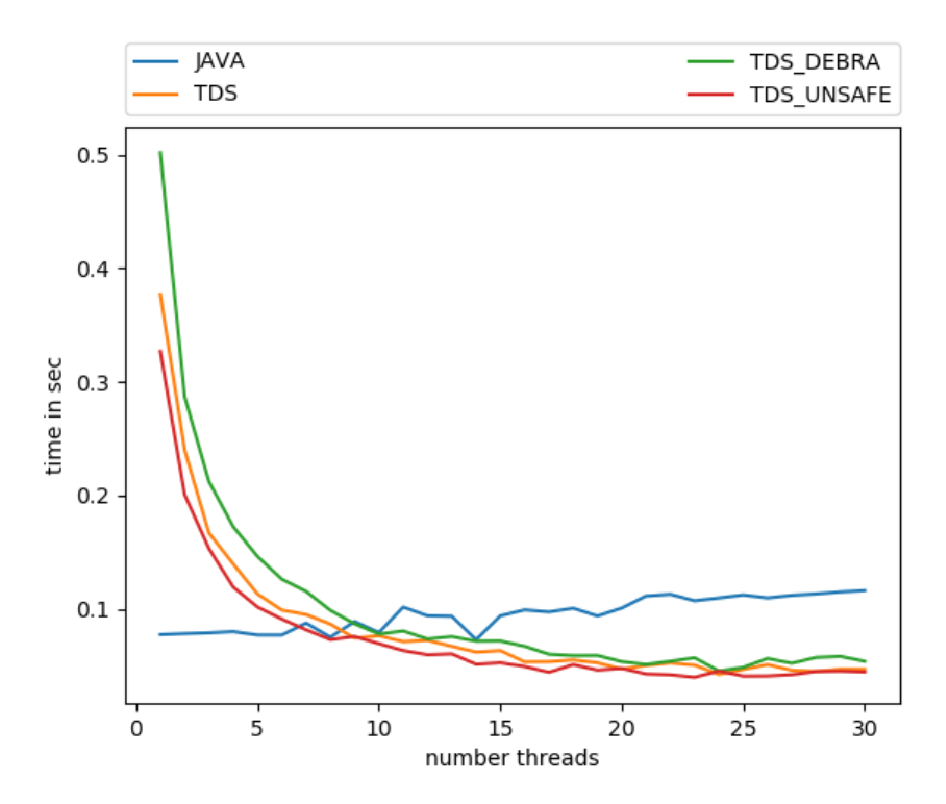
\includegraphics[scale=0.5]{50_50_times}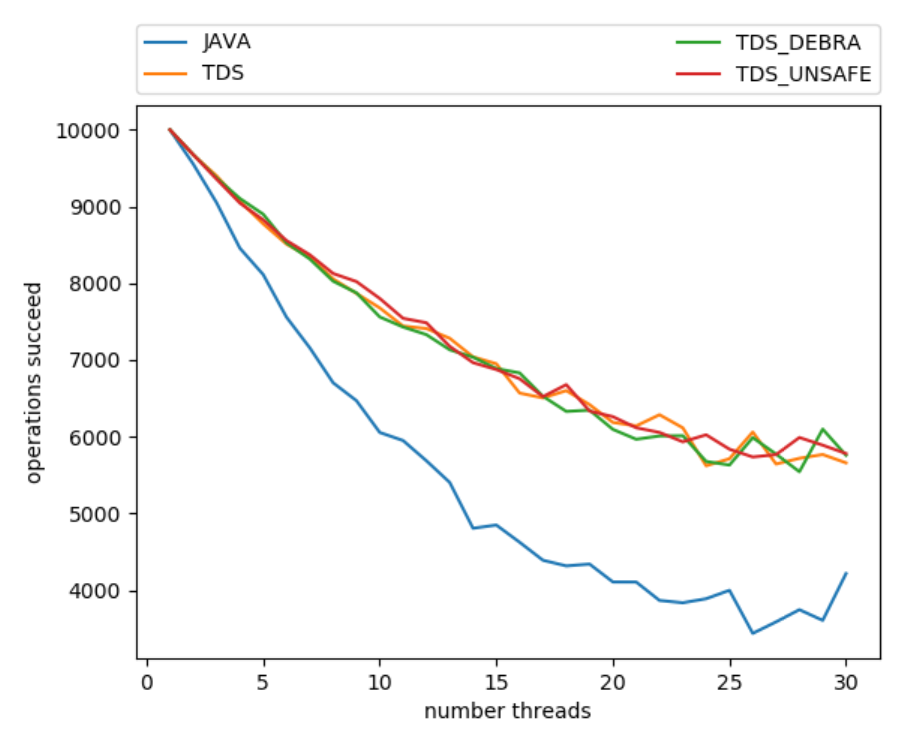
\includegraphics[scale=0.5]{50_50_succ_ops}

\subparagraph{inserts case (all tasks are inserts)\protect \\
}

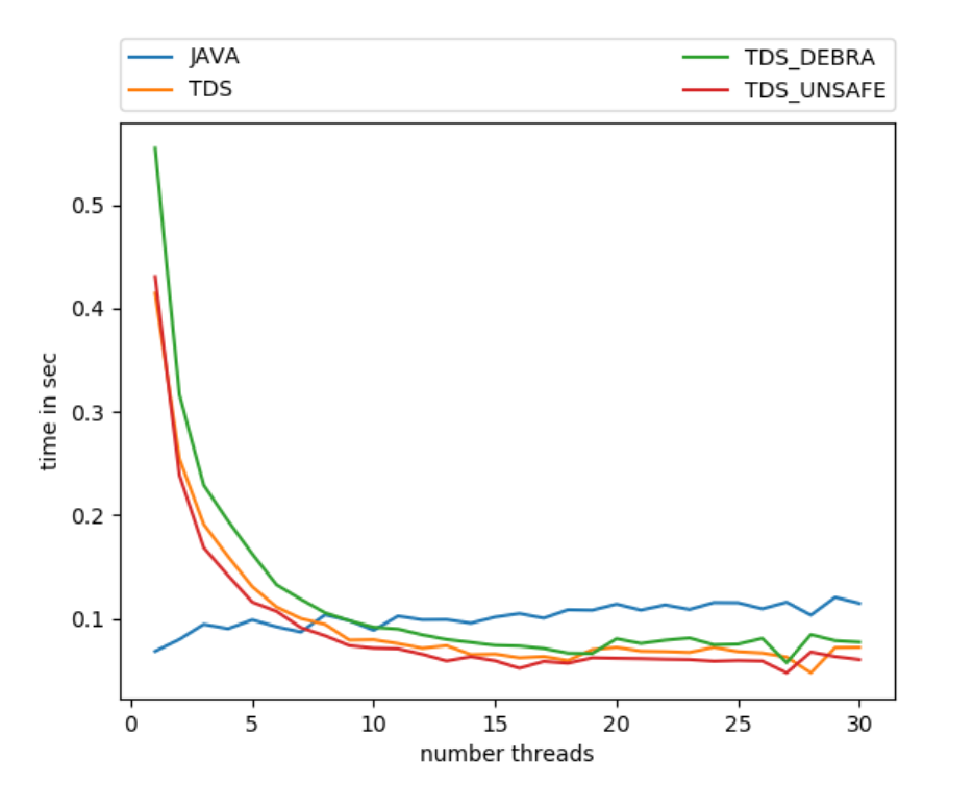
\includegraphics[scale=0.5]{100_inserts_times} 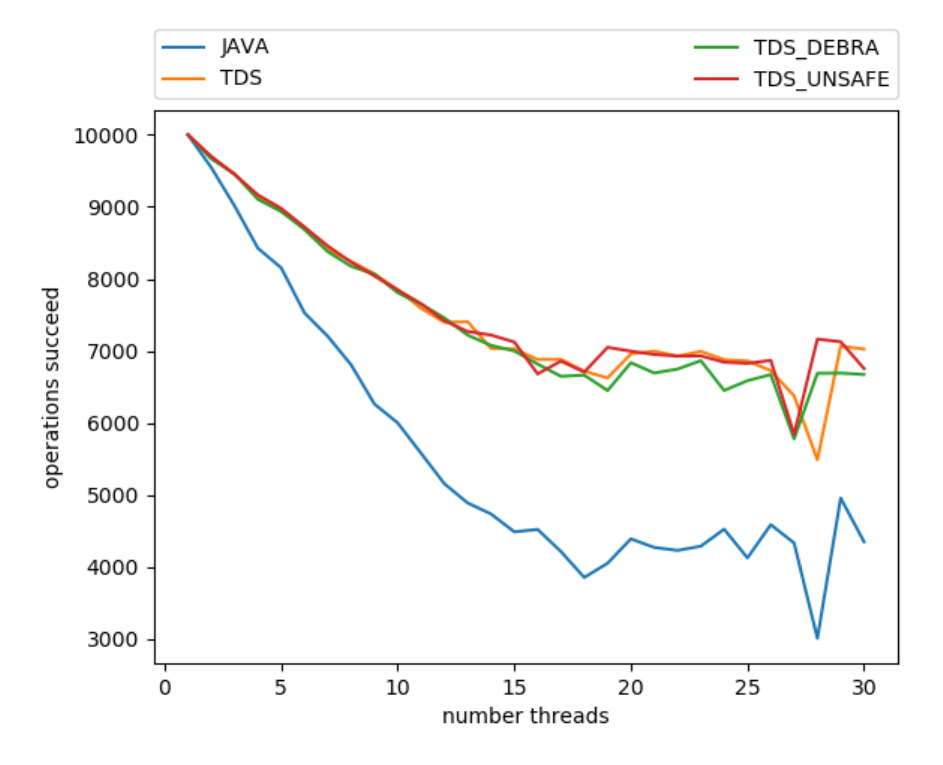
\includegraphics[scale=0.5]{100_inserts_succ_ops}

\subsection{Conclusions}
\begin{enumerate}
\item We can see that there is not a big difference between the mixed case
and the inserts case. This behavior makes sense, because there is
not a big difference between the two operations in the aspect of the
algorithm.
\item We see that when we run with more threads, more operations fail due
to transaction abort, as we would expect.
\item We can see that in terms of performance, the CPP implementation is
doing better then the JAVA implementation, when running with more
then \textasciitilde{}10 threads. It is important to mention that
we suspected that maybe for some reason the JAVA implementation is not running in parallel. To check this option, we added
print commands inside the workers code and made sure the messages
were printed alternately. For that reason we believe the JAVA implementation
does run in pararllel. Understanding the differences between the implementations
might be tricky, because there are many aspects of differences between
JAVA and CPP. But, since we see that our CPP implementation runs faster
than the JAVA implementation from {[}1{]} only after using a few threads,
and regardless to the caring of memory leak in the CPP code, we assume
this gap is more attached with the general differences between JAVA
and CPP and is not necessarily directly related to the memory cleaning.
\item It seems that there are not dramatic differences between the CPP implementations.
Yet, the experiments above shows that in general, running in unsafe
mode is faster then running in the non leaking mode, probably due
to the clear overhead of ensuring the safetiness of the second. Maybe
more surprising, is that using debra is a bit slower then using the
safe mode. Maybe this fact is related to general overhead of Debra
implementation as it uses more complicated methods.
\end{enumerate}

\section{Future Work}
\begin{enumerate}
\item Add template wrapper for all of our structs (INdexNode, Qnode,…) 
\end{enumerate}
\bibliographystyle{plain}
\bibliography{bibfile}

\end{document}
